% ================================== HEADER ====================================
\documentclass{article}           % Sets style/look of many things.
% \documentclass{report}          % part, chapters, front page etc.
\usepackage{exsheets}
\usepackage[utf8]{inputenc}       % Encoding of input files UTF-8
\usepackage[T1]{fontenc}
\usepackage[scaled]{beramono}     % Font
\usepackage{color}                % Color text
\usepackage{titlesec}             % Select alternative section titles
\usepackage{fancyvrb}
\usepackage{verbatim}             % Comment environment
\usepackage{listings}             % Format and render text/code etc.
\usepackage{minted}               % Much better syntax highlighting
\usepackage{float}                % Control of floating environment/figure
\usepackage{graphicx,  subfigure} % Better figures, graphics, units etc.
\usepackage{multicol}             % Multiple columns
\usepackage{amsmath}              % Math: Equation, split, align etc.
\usepackage{siunitx}              % SI units
\usepackage{mathtools}            % Different math tools to use with amsmath
\usepackage{amssymb}              % Math symbols
\usepackage[
    colorlinks,
    citecolor=black,              % I like links with standard black color
    filecolor=black,
    linkcolor=black,
    urlcolor=black
]{hyperref}                       % Links in TOC etc.
\usepackage[all]{hypcap}          % Better links to floating environment

\usepackage{tabto}
\newcommand\marginsymbol[1][0pt]{%
  \tabto*{0cm}\makebox[\dimexpr-1cm-#1\relax][r]{$\mathbb{P}$}\tabto*{\TabPrevPos}}

\renewcommand{\thesubsection}{\thesection.\alph{subsection}}
\title{\vspace{-2cm}INF3490/INF4490 Exercises - Week 3}
\author{Eivind Samuelsen, Ole Herman S. Elgesem}
\date{\today}

% Removing paragraph indents is sometimes useful:
\setlength\parindent{0pt}

% Make margins smaller to fit more figures, tables etc on page: (optional)
\addtolength{\oddsidemargin}{-1.0in}
\addtolength{\evensidemargin}{-1.0in}
\addtolength{\textwidth}{2.0in}
\addtolength{\topmargin}{-0.8in}
\addtolength{\textheight}{1.6in}
% ==============================================================================

% ================================= DOCUMENT ===================================
\begin{document}
    \renewcommand\marginsymbol[1][0pt]{%
  \tabto*{0cm}\makebox[-1cm][c]{$\mathbb{P}$}\tabto*{\TabPrevPos}}

\maketitle
\(\mathbb{P}\) marks the programming exercises, we strongly recommend using
the python programming language for these. Exercises may be added/changed
after publishing.


\section{Pareto Optimality}
\begin{figure}[H]
  \centering
  \begin{minipage}[b]{0.45\textwidth}
    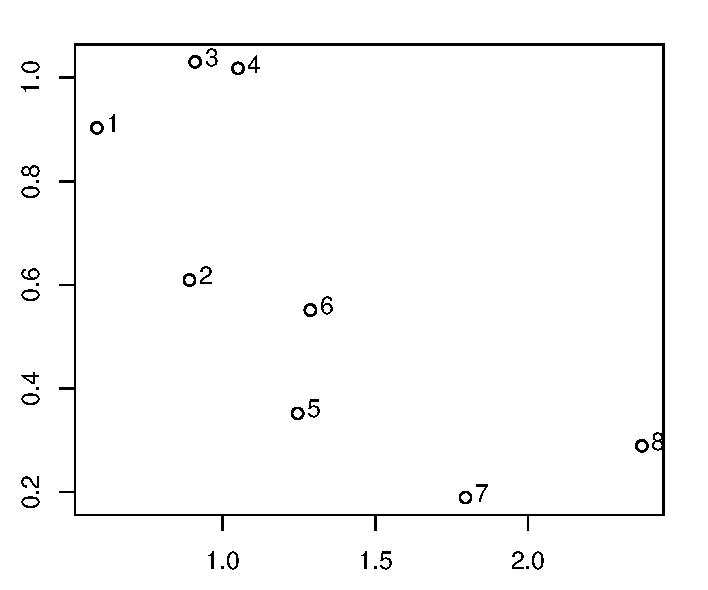
\includegraphics[width=\textwidth]{front_points_1.pdf}
    \caption{a}
  \end{minipage}
  \hfill
  \begin{minipage}[b]{0.45\textwidth}
    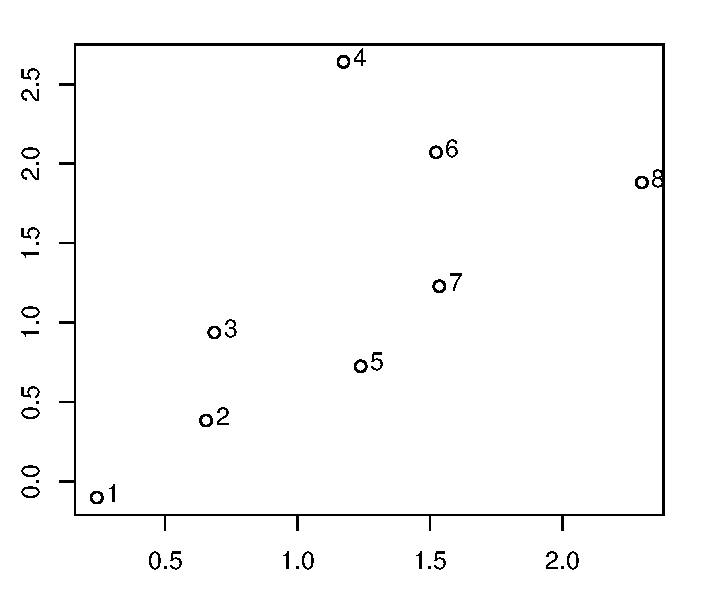
\includegraphics[width=\textwidth]{front_points_2.pdf}
    \caption{b}
  \end{minipage}
\end{figure}

For figure a and b above, find the Pareto optimal set when
\begin{itemize}
    \item Minimizing both \(f_1\) and \(f_2\)
    \item Minimizing \(f_1\), maximizing \(f_2\)
    \item Maximizing \(f_1\), minimizing \(f_2\)
    \item Maximizing both \(f_1\) and \(f_2\)
\end{itemize}
\section{Weighted sum}
In figures a and b, what would be the maximum point when using weighted sum:
\begin{itemize}
    \item \(w_1 = 1\),  \(w_2 = 1\)
    \item \(w_1 = -1\), \(w_2 = 1\)
\end{itemize}
\section{Hybrid Algorithm}
Why can hybrid algorithms make it harder to maintain diversity?
\section{Measuring algorithm performance}
Why is it usually better to use the number of fitness function evaluations as a time measure,
rather than the number of generations, or the amount of CPU time spent?

\section*{Contact and Github}
Corrections of grammar, language, notation or suggestions for improving this material are appreciated.
E-mail me at \href{mailto:olehelg@uio.no}{\textbf{olehelg@uio.no}} or use \href{https://github.com/olehermanse/INF3490-AI_Machine_Learning}{\textbf{GitHub}} to submit an issue or create a pull request.
The \href{https://github.com/olehermanse/INF3490-AI_Machine_Learning}{\textbf{GitHub repository}} contains all source code for assignments, exercises, solutions, examples etc.
As many people have been involved with writing and updating the course material, they are not all listed as authors here.
For a more complete list of authors and contributors see the \href{https://github.com/olehermanse/INF3490-AI_Machine_Learning/blob/master/README.md}{\textbf{README}}.

\end{document}
% ==============================================================================
